\documentclass[12pt,a4paper]{article}
\usepackage[utf8]{inputenc}
\usepackage[italian]{babel}
\usepackage{geometry}
\geometry{a4paper, margin=2cm}
\usepackage{graphicx}
\usepackage{float}
\usepackage{hyperref}
\usepackage{booktabs}
\usepackage{array}
\usepackage{longtable}
\usepackage{multirow}
\usepackage[table]{xcolor} 
\usepackage{listings}
\usepackage{enumitem}
\usepackage{titlesec}
\usepackage{fontenc}
\usepackage{amsmath}
\usepackage{amssymb}
\usepackage{caption}
\usepackage{subcaption}
\usepackage{tikz}
\usepackage[bottom]{footmisc}
\usepackage{tcolorbox}
\usepackage{fancyhdr}
\tcbuselibrary{skins,breakable}
\usepackage{soul}

\definecolor{WattOrange}{RGB}{230, 76, 40}

\pagestyle{fancy}
\fancyhf{}
\fancyhead[L]{\textbf{\textcolor{WattOrange}{WattGuard}}}
\fancyhead[R]{\textbf{\thepage}}
\renewcommand{\headrulewidth}{0.4pt}

\newcommand{\ProjectTitle}{WattGuard}

\newenvironment{rfList}{\begin{itemize}[leftmargin=2cm, label={}]}{\end{itemize}}
\newcommand{\rfItem}[1]{\item \textbf{#1:}}

\newenvironment{rnfList}{\begin{itemize}[leftmargin=2cm, label={}]}{\end{itemize}}
\newcommand{\rnfItem}[1]{\item \textbf{#1:}}

\hypersetup{
    colorlinks=true,
    linkcolor=blue,
    urlcolor=blue,
    citecolor=blue
}

\lstset{
    basicstyle=\ttfamily\small,
    breaklines=true,
    frame=single,
    numbers=left,
    numberstyle=\tiny,
    keywordstyle=\color{blue},
    commentstyle=\color{green!50!black},
    stringstyle=\color{red!50!black},
    tabsize=2
}

\begin{document}

\begin{titlepage}
    \noindent
\includegraphics[width=0.25\textwidth]{../images/logoUni.png}
    
    \vspace{2cm}
    
    \noindent\textbf{Progetto:}
    \vspace{0.5cm}
    \begin{center}
        {\huge \textbf{\ProjectTitle}}
    \end{center}
    
    \vspace{2cm}
    
    \noindent\textbf{Titolo del documento:}
    \vspace{0.5cm}
    \begin{center}
        {\LARGE \textbf{Analisi e Progettazione}}
    \end{center}
    
    \vspace{2cm}
    
    \noindent\textbf{Document Info}\\[0.5cm]
    \begingroup
    \renewcommand{\arraystretch}{1.5}
    \setlength{\tabcolsep}{6pt}
    \begin{tabular}{|p{2.8cm}|p{6.5cm}|p{3cm}|p{2.5cm}|}
        \hline
        \cellcolor{WattOrange!60}\textbf{Doc. Name} & 
        D3-\ProjectTitle-DescrizioneProgetto & 
        \cellcolor{WattOrange!60}\textbf{Doc. Number} & 
        D3 V1.0 \\
        \hline
        \cellcolor{WattOrange!60}\textbf{Description} & 
        \multicolumn{3}{l|}{Documento di analisi e progettazzione} \\
        \hline
    \end{tabular}
    \endgroup
    
    \vfill
    
    \hfill
    \begin{minipage}{0.35\textwidth}
        \centering
        \textbf{Authors}\\[0.3cm]
        \begin{tabular}{c c}
            Alessio Pesaresi & 251783 \\
            Michele Porcellato & 254581 \\
            Marco Piovesan & 255380 \\
        \end{tabular}
    \end{minipage}
\end{titlepage}


\tableofcontents
\newpage
\section{Analisi dei componenti}
    Nel presente capitolo viene presentata l'architettura in termini di componenti interni al sistema \texttt{WattGuard}, definiti sulla base dei requisiti analizzati in precedenza. L'architettura adotta un modello a dati centralizzato: tutti i dati (provenienti dai sensori e dalle API meteo) vengono prima acquisiti e resi persistenti nel database, per poi essere messi a disposizione di tutti gli altri componenti che li richiedono esclusivamente attraverso il database stesso.

    \textit{Nota di conformit\`a all'implementazione.} I nomi di campi e riferimenti usati nel documento corrispondono ai nomi reali dei modelli Mongoose implementati: \texttt{building} (non \texttt{buildingId}), \texttt{sensor} (non \texttt{sensorId}), \texttt{metadata.sensor} e \texttt{metadata.building} (non \texttt{metadata.sensorId} / \texttt{metadata.buildingId}). Nelle risposte JSON delle API l'identificativo \`e esposto come \texttt{\_id} (con \texttt{self} come link canonico) e i riferimenti sono risolti via \texttt{populate}.

\subsection{Definizione dei componenti}
    Definiamo di seguito i componenti del sistema con le relative funzionalità.
    
    \subsubsection{Gestione autenticazione}
        \subsubsection*{Descrizione} 
            Il componente si occupa della funzionalità di autenticazione degli utenti (Amministratore e Operatore Tecnico) tramite credenziali locali (email/password con hashing) o tramite autenticazione federata con Google (\texttt{SSO}). Include le funzionalità di login e reset della password. Il logout \`e esclusivamente client-side (rimozione del JWT da \texttt{localStorage}, nessun endpoint di revoca server-side perch\'e i token sono stateless con scadenza di 8 ore). L'onboarding dei nuovi operatori avviene tramite invite-link e non tramite credenziali temporanee generate.
        \subsubsection*{Interfaccia richiesta - Credenziali locali:}
            Riceve dall'utente l'inserimento di email e password per l'accesso al sistema. Le password sono memorizzate utilizzando algoritmi di hashing robusti (bcrypt, costo 10) con salt individuale.
        \subsubsection*{Interfaccia richiesta - Autenticazione Google:}
            Riceve l'autorizzazione all'accesso al sistema proveniente dall'\texttt{SSO} di Google, previo controllo delle credenziali inserite dall'utente nei sistemi Google. L'account Google deve essere pre-registrato tramite invito: in caso contrario l'accesso \`e rifiutato (\texttt{oauth\_no\_account}). Il login locale e quello Google condividono lo stesso endpoint \texttt{POST /auth/session}.
        \subsubsection*{Interfaccia fornita - Richiesta a Google:}
            Provvede alla configurazione esposta da \texttt{GET /auth/google/config}; la verifica del token \texttt{idToken} avviene server-side con \texttt{google-auth-library} (nessun redirect URI/secret dedicato).
        \subsubsection*{Interfaccia fornita - Autenticazione e ruolo:}
            Fornisce il token JWT (\texttt{Authorization: Bearer}, scadenza 8 ore) e il ruolo dell'utente (Amministratore o Operatore), permettendo l'accesso alle funzionalità corrispondenti.
        \subsubsection*{Interfaccia fornita - Attivazione credenziali:}
            L'amministratore crea un invito (\texttt{POST /invites}, scadenza 7 giorni) e il nuovo utente lo accetta tramite \texttt{PATCH /invites/:id} impostando la password locale oppure collegando l'account Google; non vengono generate n\'e inviate password in chiaro.

    \subsubsection{Gestione database}
        \subsubsection*{Descrizione} 
            Punto centrale di archiviazione e unico punto di accesso ai dati (unica connessione Mongoose verso MongoDB). Gestisce i dati storici, le configurazioni di edifici e sensori, le credenziali locali, i log di sistema e i report. Non \`e implementato alcun backup automatico giornaliero con retention di 30 giorni: la retention configurabile (\texttt{database.dataRetentionDays}, default 365 giorni) si applica alle rilevazioni tramite TTL sulla collezione time-series \texttt{sensorreadings}. Tutti i componenti del sistema richiedono i dati esclusivamente attraverso questo componente.
        \subsubsection*{Interfaccia richiesta - Dati sensori:}
            Riceve le rilevazioni dei sensori per l'archiviazione storica.
        \subsubsection*{Interfaccia richiesta - Dati meteo:}
            Riceve i dati della temperatura esterna per l'archiviazione e il successivo utilizzo.
        \subsubsection*{Interfaccia richiesta - Dati modificati:}
            Riceve le modifiche apportate ai dati per la persistenza.
        \subsubsection*{Interfaccia fornita - Dati storici:}
            Fornisce le rilevazioni archiviate per l'intervallo temporale selezionato.
        \subsubsection*{Interfaccia fornita - Dati in tempo reale:}
            Fornisce le ultime rilevazioni disponibili per il monitoraggio live.
        \subsubsection*{Interfaccia fornita - Temperatura esterna:}
            Fornisce i dati meteo archiviati per l'analisi comparativa dell'efficienza termica.
        \subsubsection*{Interfaccia fornita - Metadati edificio:}
            Fornisce i dettagli strutturali degli edifici (nome, indirizzo, superficie, tipologia impianto) e la configurazione dei sensori associati.
        \subsubsection*{Interfaccia fornita - Soglie personalizzate:}
            Fornisce i limiti configurati per temperatura e consumo.
        \subsubsection*{Interfaccia fornita - Validazione email:}
            Verifica l'unicità dell'indirizzo email nel database.
        \subsubsection*{Interfaccia fornita - Dati per backup:}
            Fornisce l'intero set di dati per l'esportazione on-demand tramite \texttt{GET /backups} (riservato all'amministratore). Non include la collezione \texttt{sensorreadings}, non prevede scheduling automatico, storage dedicato n\'e ripristino.

    \subsubsection{Acquisizione dati real-time}
        \subsubsection*{Descrizione}
            Gestisce la ricezione delle misurazioni dai termometri smart e dai contatori connessi con una frequenza media di 90 secondi (\texttt{transmissionInterval}, default 90, configurabile tra 10 e 3600 secondi). Riceve i pacchetti dati dai dispositivi \texttt{IoT} e li rende disponibili esclusivamente per l'archiviazione nel database. L'ingestione \texttt{MQTT} (\texttt{sensors/+/readings}) \`e disabilitata di default (\texttt{MQTT\_ENABLED=false}) e la sorgente effettivamente attiva \`e il simulatore in-process, che emette con la stessa cadenza e invoca lo stesso servizio di ingestione (scrittura time-series, deduplica soglie in transazione, denormalizzazione di \texttt{lastReading}).
        \subsubsection*{Interfaccia richiesta - Connessione sensori:}
            Riceve i pacchetti dati dai dispositivi \texttt{IoT} (termometri e contatori) tramite protocollo \texttt{MQTT}.
        \subsubsection*{Interfaccia fornita - Dati sensori:}
            Invia i dati correnti per l'archiviazione e la successiva distribuzione agli altri componenti.

    \subsubsection{Integrazione meteo}
        \subsubsection*{Descrizione}
            Si occupa di reperire i dati della temperatura ambientale esterna tramite API meteo esterne (Open-Meteo, con geocoding via Nominatim OpenStreetMap) senza scheduling orario dedicato: i dati esterni sono usati come fallback per i calcoli di efficienza quando manca un sensore \texttt{external\_temp}. Il frontend interroga direttamente \texttt{api.open-meteo.com} (coordinate di Trento hardcoded, \texttt{staleTime} 5 minuti) per l'intestazione comparativa.
        \subsubsection*{Interfaccia richiesta - API esterne:}
            Richiede dati ai provider meteo tramite chiamate \texttt{REST} (backend: archivio orario Open-Meteo; frontend: forecast corrente Open-Meteo).
        \subsubsection*{Interfaccia fornita - Dati meteo:}
            Invia i dati climatici per l'archiviazione e la successiva distribuzione agli altri componenti.

    \subsubsection{Gestione dashboard e grafici}
        \subsubsection*{Descrizione}
            Genera la panoramica dei consumi e i grafici storici aggregati. Elabora i dati grezzi per visualizzare indici di performance e andamenti temporali (orari, giornalieri e settimanali su \texttt{GET /metrics/timeseries}; giornalieri nei report; mensili e annuali non implementati). Nessuno SLO di caricamento entro 60 secondi per il 95\% delle richieste \`e misurato nell'implementazione.
        \subsubsection*{Interfaccia richiesta - Dati storici:}
            Riceve le rilevazioni archiviate per l'intervallo selezionato.
        \subsubsection*{Interfaccia richiesta - Dati in tempo reale:}
            Riceve le ultime rilevazioni disponibili con polling guidato da \texttt{settings.polling.intervalSeconds} (default 90 secondi; fallback frontend 120 secondi per le statistiche dashboard, 30 secondi di \texttt{staleTime} per il dettaglio edificio).
        \subsubsection*{Interfaccia richiesta - Temperatura esterna:}
            Riceve i dati meteo archiviati per i calcoli di efficienza.
        \subsubsection*{Interfaccia fornita - Visualizzazione:}
            Fornisce al front-end i grafici interattivi e gli indicatori disponibili in \texttt{GET /metrics} (sensori attivi/totali, allarmi attivi, consumi elettrici e gas come somma delle ultime letture; le temperature medie sono disponibili solo nel drill-down di edificio, non nei KPI aggregati).
        \subsubsection*{Interfaccia fornita - Indicatori performance:}
            Fornisce i calcoli di efficienza (\texttt{GET /buildings/:id/efficiency}) per il confronto tra edifici.

    \subsubsection{Gestione edifici e sensori}
        \subsubsection*{Descrizione}
            Gestisce l'anagrafica degli edifici pubblici (nome, indirizzo, superficie, anno costruzione, tipologia impianto) e la configurazione dei sensori associati (termometri smart e contatori). Permette di aggiungere, modificare e rimuovere edifici e sensori. Ogni modifica viene registrata con timestamp e identificativo dell'operatore.
        \subsubsection*{Interfaccia richiesta - Autorizzazione:}
            Riceve il ruolo dell'utente (\texttt{admin} o \texttt{operator}, trasportato nel claim JWT e verificato dai middleware \texttt{requireOperator}/\texttt{requireAdmin}) che segnala se l'utente ha il permesso necessario per compiere un'azione.
        \subsubsection*{Interfaccia richiesta - Metadati edificio:}
            Riceve i dettagli strutturali e la configurazione dei sensori per le operazioni di visualizzazione e modifica.
        \subsubsection*{Interfaccia fornita - Dati edificio aggiornati:}
            Invia le modifiche apportate agli edifici e ai sensori per la persistenza, con audit tramite \texttt{createdBy}/\texttt{updatedBy} e \texttt{createdAt}/\texttt{updatedAt} (nessun log versionato immutabile separato).
        \subsubsection*{Interfaccia fornita - Evento modifica:}
            Notifica ogni operazione di modifica, aggiunta o rimozione di edifici e sensori.

    \subsubsection{Sistema di allerta e notifiche}
        \subsubsection*{Descrizione}
            Monitora costantemente le rilevazioni rispetto alle soglie configurate sul sensore (\texttt{minThreshold}/\texttt{maxThreshold}) e alla soglia di efficienza (\texttt{efficiencyThresholds.minCop}, verificata da un job ogni 30 minuti su finestra 24h) e genera notifiche automatiche in caso di anomalie o malfunzionamenti. Le notifiche vengono visualizzate in un pannello dedicato con tab \texttt{active}/\texttt{acknowledged}/\texttt{resolved} e ciclo di vita \texttt{active} $\rightarrow$ \texttt{acknowledged} $\rightarrow$ \texttt{resolved} tramite \texttt{PATCH /alerts/:id}; possono essere prese in carico e chiuse dall'operatore dopo la risoluzione del problema.
        \subsubsection*{Interfaccia richiesta - Soglie personalizzate:}
            Riceve i limiti impostati (es. temperatura min/max, consumo massimo orario, variazioni anomale) dagli attributi di sensore ed edificio.
        \subsubsection*{Interfaccia richiesta - Dati in tempo reale:}
            Riceve le ultime rilevazioni disponibili per la verifica in tempo reale delle soglie, con deduplica (un solo allarme \texttt{active} per sensore/tipo).
        \subsubsection*{Interfaccia richiesta - Autorizzazione:}
            Riceve il ruolo dell'utente (\texttt{admin} o \texttt{operator}) che segnala se l'utente ha i permessi per visualizzare e gestire gli allarmi.
        \subsubsection*{Interfaccia fornita - Allarmi:}
            Genera toast in-app ed email broadcast (nessuna notifica desktop/push nativa) oltre alle voci nel pannello dedicato per la gestione degli interventi, ordinate per \texttt{createdAt} discendente lato backend.
        \subsubsection*{Interfaccia fornita - Evento allarme:}
            Notifica la generazione, la presa in carico e la chiusura di ogni allarme (con \texttt{acknowledgedBy}/\texttt{acknowledgedAt} e \texttt{resolvedBy}/\texttt{resolvedAt} come nome utente e data).

    \subsubsection{Gestione esportazione}
        \subsubsection*{Descrizione}
            Genera report riservati all'amministratore, per singoli edifici o gruppi di edifici e per periodi temporali specifici (\texttt{buildingIds}, \texttt{startDate}, \texttt{endDate}). I dati grezzi sono esportati da \texttt{GET /readings} in formato CSV e JSON; i report aggregati (riepilogo + giornaliero con grafico) sono esportati da \texttt{GET /reports} in formato PDF e XLSX. Include dati anagrafici, consumi, temperature, timestamp e anomalie a seconda della sorgente.
        \subsubsection*{Interfaccia richiesta - Dati per export:}
            Riceve i dati storici filtrati per edificio e periodo temporale.
        \subsubsection*{Interfaccia richiesta - Autorizzazione esportazione:}
            Riceve il ruolo dell'utente e verifica che sia Amministratore (\texttt{requireAdmin}) per esportare i dati.
        \subsubsection*{Interfaccia fornita - Download:}
            Fornisce il trigger per il download immediato dei dati filtrati. Il CSV \`e formattato correttamente per l'importazione in Excel.

    \subsubsection{Gestione utenti}
        \subsubsection*{Descrizione}
            Permette all'amministratore comunale di gestire gli account degli operatori tecnici. Si occupa della creazione (esclusivamente tramite inviti, nessuna \texttt{POST /users}), modifica (\texttt{role}, \texttt{isDisabled}), eliminazione e gestione dei permessi dei profili utente, con protezione anti auto-modifica. Il sistema invia automaticamente una email all'operatore con il link di invito e le istruzioni per il primo accesso (impostazione password o collegamento Google); non vengono inviate credenziali in chiaro.
        \subsubsection*{Interfaccia richiesta - Validazione email:}
            Verifica l'unicità dell'indirizzo email inserito prima di procedere alla creazione dell'invito.
        \subsubsection*{Interfaccia richiesta - Template messaggio:}
            Riceve il template dell'email da inviare al nuovo operatore.
        \subsubsection*{Interfaccia fornita - Gestione account:}
            Fornisce le funzionalità per inserire email e permessi dell'utente.
        \subsubsection*{Interfaccia fornita - Credenziali generate:}
            Fornisce l'invito con token (hash SHA-256, scadenza 7 giorni) accettabile dal nuovo operatore/amministratore tramite \texttt{PATCH /invites/:id}; se l'invio email fallisce, l'invito viene annullato.
        \subsubsection*{Interfaccia fornita - Richiesta invio email:}
            Richiede l'invio effettivo dell'email di benvenuto con link \texttt{/accept-invite?token=}.
        \subsubsection*{Interfaccia fornita - Evento gestione utenti:}
            Notifica ogni operazione di creazione, modifica o eliminazione di account.

    \subsubsection{Motore di ricerca edifici}
        \subsubsection*{Descrizione}
            Implementa la logica di ricerca degli edifici pubblici monitorati. L'API (\texttt{GET /buildings}) permette di filtrare in combinazione AND per nome, indirizzo, zona geografica, tipologia di struttura (per esempio scuola, ospedale, ecc.) e stato, con paginazione, ordinamento e indici dedicati. Il componente di ricerca del frontend inoltra al server il solo filtro di stato e applica gli altri filtri (nome, indirizzo, tipologia) lato client; nessun campo di ricerca per zona \`e esposto nella UI. Nessuno SLO di completamento entro 10 secondi \`e misurato nell'implementazione.
        \subsubsection*{Interfaccia richiesta - Dati anagrafici:}
            Riceve la lista degli edifici che corrispondono ai criteri inseriti.
        \subsubsection*{Interfaccia fornita - Risultati ricerca:}
            Restituisce una lista di edifici completa di dettagli quali superficie, stato operativo e tipologia di impianto.

    \subsubsection{Gestione autorizzazioni}
        \subsubsection*{Descrizione}
            Determina a quali funzionalità un utente può accedere in base al ruolo assegnato (Operatore o Amministratore). Controlla, ad esempio, se un utente ha il permesso di esportare dati o gestire altri utenti. Non \`e usata alcuna bitmask: il ruolo \`e un enum (\texttt{admin} $|$ \texttt{operator}) trasportato nel JWT e verificato dai middleware \texttt{requireOperator} (\texttt{admin} + \texttt{operator}) e \texttt{requireAdmin} (solo \texttt{admin}).
        \subsubsection*{Interfaccia richiesta - Ruolo utente:}
            Riceve l'identità certificata e il ruolo dell'utente loggato.
        \subsubsection*{Interfaccia fornita - Bit di autorizzazione:}
            Fornisce l'esito dei controlli di ruolo che determinano se l'utente ha il permesso necessario per compiere un'azione.

    \subsubsection{Analisi comparativa}
        \subsubsection*{Descrizione}
            Componente dedicato al confronto delle performance tra diversi edifici. Permette di selezionare al massimo 3 edifici (\texttt{MAX\_COMPARE\_BUILDINGS=3}, limite rigido) per confrontarne superficie, sensori attivi, consumo corrente, consumo per m$^2$, tipologia, anno, impianto, zona ed efficienza (COP, dispersione, kWh totali). Non sono implementati costi stimati, temperature medie nella vista comparativa n\'e badge di edificio pi\`u/meno efficiente: i valori sono solo affiancati.
        \subsubsection*{Interfaccia richiesta - Indicatori performance:}
            Riceve i calcoli di efficienza relativi agli edifici selezionati.
        \subsubsection*{Interfaccia richiesta - Metadati edificio:}
            Riceve i dettagli anagrafici degli edifici da confrontare.
        \subsubsection*{Interfaccia fornita - Confronto visivo:}
            Genera tabelle comparative e grafici affiancati per evidenziare gli edifici più e meno efficienti.

    \subsubsection{Servizio comunicazioni (email)}
        \subsubsection*{Descrizione}
            Gestisce l'invio automatico di comunicazioni verso l'esterno tramite il provider Resend via HTTP (non via server SMTP dedicato). È responsabile della spedizione delle email con il link di invito ai nuovi operatori, dei link per il reset della password e delle notifiche di allarme (creazione/risoluzione, in modalit\`a fire-and-forget se \texttt{notifications.emailEnabled} \`e attivo).
        \subsubsection*{Interfaccia richiesta - Richiesta invio:}
            Riceve la richiesta di invio email con i dettagli del destinatario e il contenuto.
        \subsubsection*{Interfaccia fornita - Invio mail:}
            Si interfaccia con le API Resend per il recapito effettivo dei messaggi agli indirizzi email degli utenti.
        \subsubsection*{Interfaccia fornita - Template messaggi:}
            Fornisce i template predefiniti per le email di benvenuto (con link di invito), di reset password e di notifica allarme.

\newpage
\subsection{Diagramma dei componenti}
    Viene riportato di seguito un diagramma complessivo di tutti i componenti di sistema e le loro interconnessioni descritte in precedenza. Come si evince dal diagramma, il componente ``Gestione database'' rappresenta il punto centrale di raccolta e distribuzione dei dati, garantendo che tutti gli altri componenti accedano ai dati esclusivamente attraverso di esso.
    \begin{figure}[H]
        \centering
        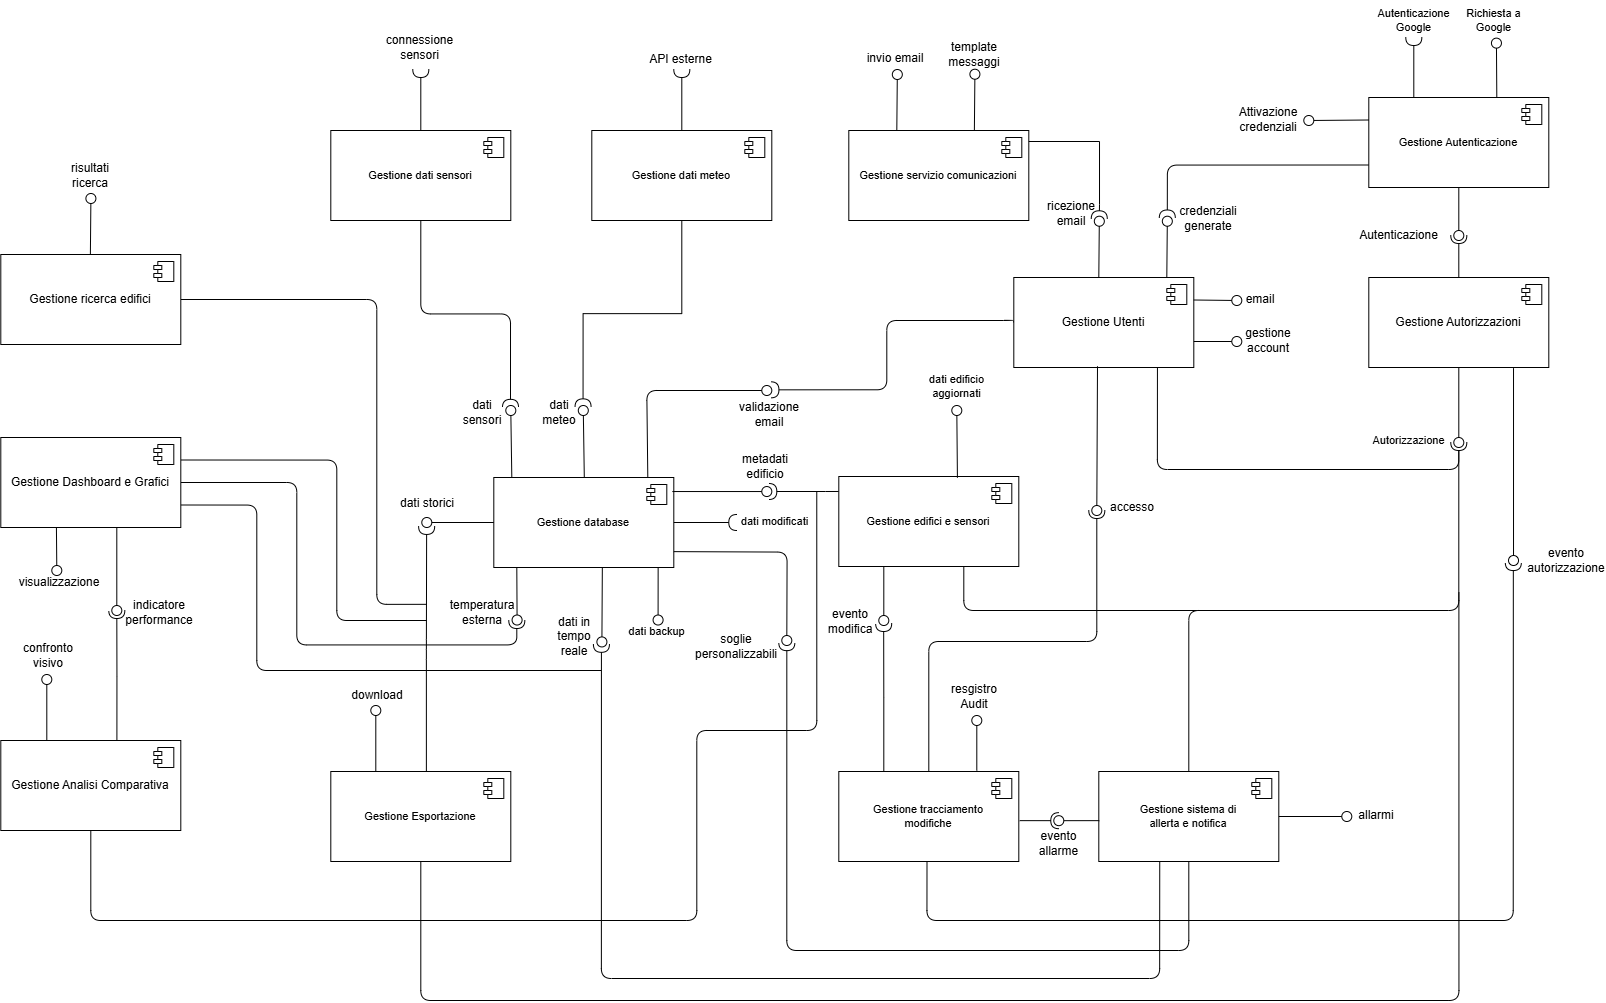
\includegraphics[width=1\textwidth]{../images/ComponentDiagram/ComponentDiagram.png}
        \caption{Diagramma dei componenti di \texttt{WattGuard}}
    \end{figure}
\section{Diagramma delle classi}
\label{ch:diagrammaClassi}

\subsection{Definizione delle classi}

 Le figure seguenti riportano i nomi reali dei campi Mongoose implementati. Nelle risposte JSON l'identificativo \`e esposto come \texttt{\_id} (con \texttt{self} come link canonico). 
    Ogni classe riporta oltre agli attributi anche i metodi (operazioni). La mappatura completa metodo $\rightarrow$ endpoint REST \`e nel capitolo~\ref{ch:dalClassDiagramAlleAPI}.

    \subsection*{1. Utente (\texttt{User})}
        La classe \texttt{Utente} rappresenta qualsiasi utente del sistema. Il ruolo viene memorizzato nell'attributo \texttt{role} (enum \texttt{admin} o \texttt{operator}): l'operatore tecnico gestisce edifici, sensori e allarmi mentre l'amministratore possiede il controllo totale (gestione utenti, inviti, esportazione dati, configurazione di sistema oltre ai privielgi dell'operatore tecnico).
        \begin{figure}[H]
            \centering
            \includegraphics[width=0.5\textwidth]{../images/ClassDiagram/ClassiWattguard-Utente.png}
            \caption{Classe \texttt{Utente}: attributi e metodi}
        \end{figure}

    \subsection*{2. Invito (\texttt{Invite})}
        La classe \texttt{Invito} rappresenta l'invito inviato via email a un nuovo utente, con il relativo token e la scadenza (7 giorni). Permette all'amministratore di creare gli account senza condividerne le credenziali.
        \begin{figure}[H]
            \centering
            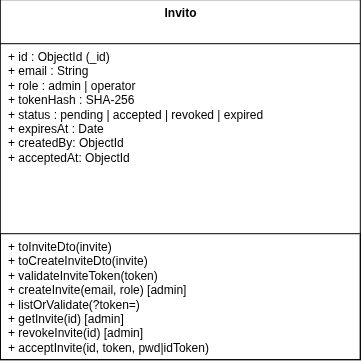
\includegraphics[width=0.5\textwidth]{../images/ClassDiagram/ClassiWattguard-Invito.png}
            \caption{Classe \texttt{Invito}: attributi e metodi}
        \end{figure}

    \subsection*{3. TokenResetPassword (\texttt{PasswordResetToken})}
        La classe \texttt{TokenResetPassword} rappresenta il token monouso generato per la procedura di reset della password. Il token scade dopo 1 ora (durata impostata dal service).
        \begin{figure}[H]
            \centering
            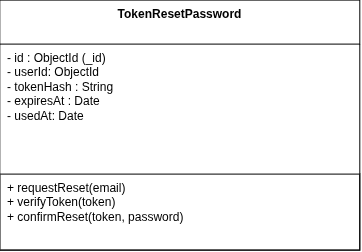
\includegraphics[width=0.5\textwidth]{../images/ClassDiagram/ClassiWattguard-TokenResetPassword.png}
            \caption{Classe \texttt{TokenResetPassword}: attributi e metodi}
        \end{figure}

    \subsection*{4. Edificio (\texttt{Building})}
        La classe \texttt{Edificio} rappresenta la struttura pubblica monitorata dal sistema. Oltre ai dati anagrafici e strutturali, memorizza la posizione geografica come punto \texttt{GeoJSON} (longitudine/latitudine) e conserva il riferimento alla propria tipologia.
        \begin{figure}[H]
            \centering
            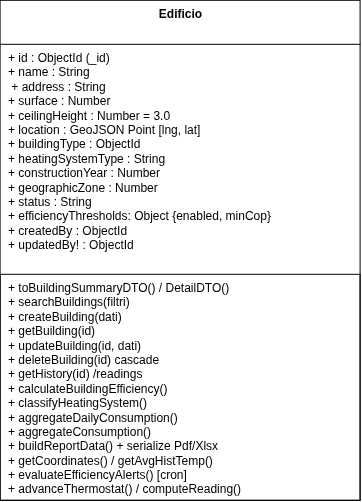
\includegraphics[width=0.5\textwidth]{../images/ClassDiagram/ClassiWattguard-Edificio.png}
            \caption{Classe \texttt{Edificio}: attributi e metodi}
        \end{figure}

    \subsection*{5. TipologiaEdificio (\texttt{BuildingType})}
        La classe \texttt{TipologiaEdificio} rappresenta le categorie di edifici (ad esempio ``scuola'', ``ufficio'', ``palestra''). Il nome è univoco; una tipologia può essere eliminata solo se non è più utilizzata da alcun edificio.
        \begin{figure}[H]
            \centering
            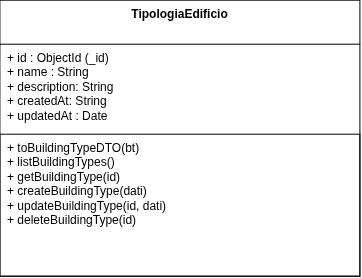
\includegraphics[width=0.5\textwidth]{../images/ClassDiagram/ClassiWattguard-TipologiaEdificio.png}
            \caption{Classe \texttt{TipologiaEdificio}: attributi e metodi}
        \end{figure}

    \subsection*{6. Sensore (\texttt{Sensor})}
        La classe \texttt{Sensore} rappresenta un dispositivo IoT installato in un edificio. Il riferimento all'edificio \`e memorizzato nel campo \texttt{building} (nome reale nel codice). La tipologia è un attributo enumerato (temperatura interna, temperatura esterna, contatore elettrico, contatore gas); le soglie di allarme \texttt{minThreshold} e \texttt{maxThreshold} sono attributi del sensore stesso. L'ultima rilevazione è memorizzata in forma denormalizzata nell'attributo \texttt{lastReading} per garantire letture immediate, mentre lo storico completo è nella classe \texttt{Rilevazione}.
        \begin{figure}[H]
            \centering
            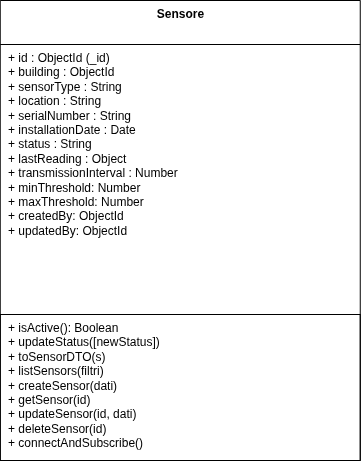
\includegraphics[width=0.5\textwidth]{../images/ClassDiagram/ClassiWattguard-Sensore.png}
            \caption{Classe \texttt{Sensore}: attributi e metodi}
        \end{figure}


    \subsection*{7. Rilevazione (\texttt{SensorReading})}
        La classe \texttt{Rilevazione} rappresenta una singola misurazione effettuata da un sensore in un determinato istante. È una collezione che mantiene lo storico dei dati necessario alle analisi di andamento, efficienza e all'esportazione. Un TTL di 365 giorni rimuove automaticamente le rilevazioni pi\`u vecchie.
        \begin{figure}[H]
            \centering
            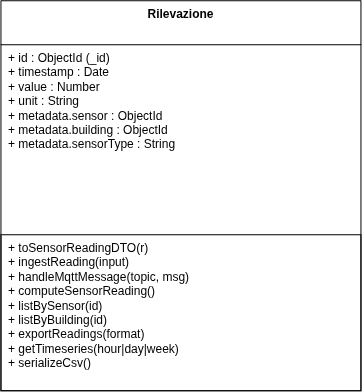
\includegraphics[width=0.5\textwidth]{../images/ClassDiagram/ClassiWattguard-Rilevazione.png}
            \caption{Classe \texttt{Rilevazione}: attributi e metodi}
        \end{figure}

    \subsection*{8. Allarme (\texttt{Alert})}
        La classe \texttt{Allarme} rappresenta una notifica generata automaticamente dal sistema quando una rilevazione supera le soglie configurate sul sensore oppure quando viene rilevata un'anomalia di efficienza (COP sotto soglia). 
        \begin{figure}[H]
            \centering
            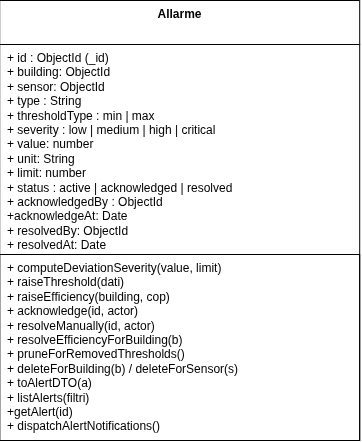
\includegraphics[width=0.5\textwidth]{../images/ClassDiagram/ClassiWattguard-Allarme.png}
            \caption{Classe \texttt{Allarme}: attributi e metodi}
        \end{figure}

    \subsection*{9. Configurazione Sistema (\texttt{SystemConfig})}
        La classe \texttt{ConfigurazioneSistema} è un documento \emph{singleton} solo per convenzione applicativa che conserva la configurazione globale del sistema (intervallo di polling del frontend, abilitazione delle notifiche email, giorni di conservazione dei dati storici).
        \begin{figure}[H]
            \centering
            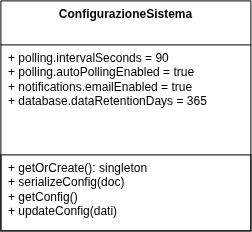
\includegraphics[width=0.5\textwidth]{../images/ClassDiagram/ClassiWattguard-ConfigurazioneSistema.png}
            \caption{Classe \texttt{ConfigurazioneSistema}: attributi e metodi}
        \end{figure}

\newpage

\subsection{Diagramma delle classi complessivo}
    Di seguito il diagramma delle classi complessivo con tutte le classi presentate e le relative relazioni (da rigenerare in base alle definizioni corrette).
    \begin{figure}[H]
        \centering
        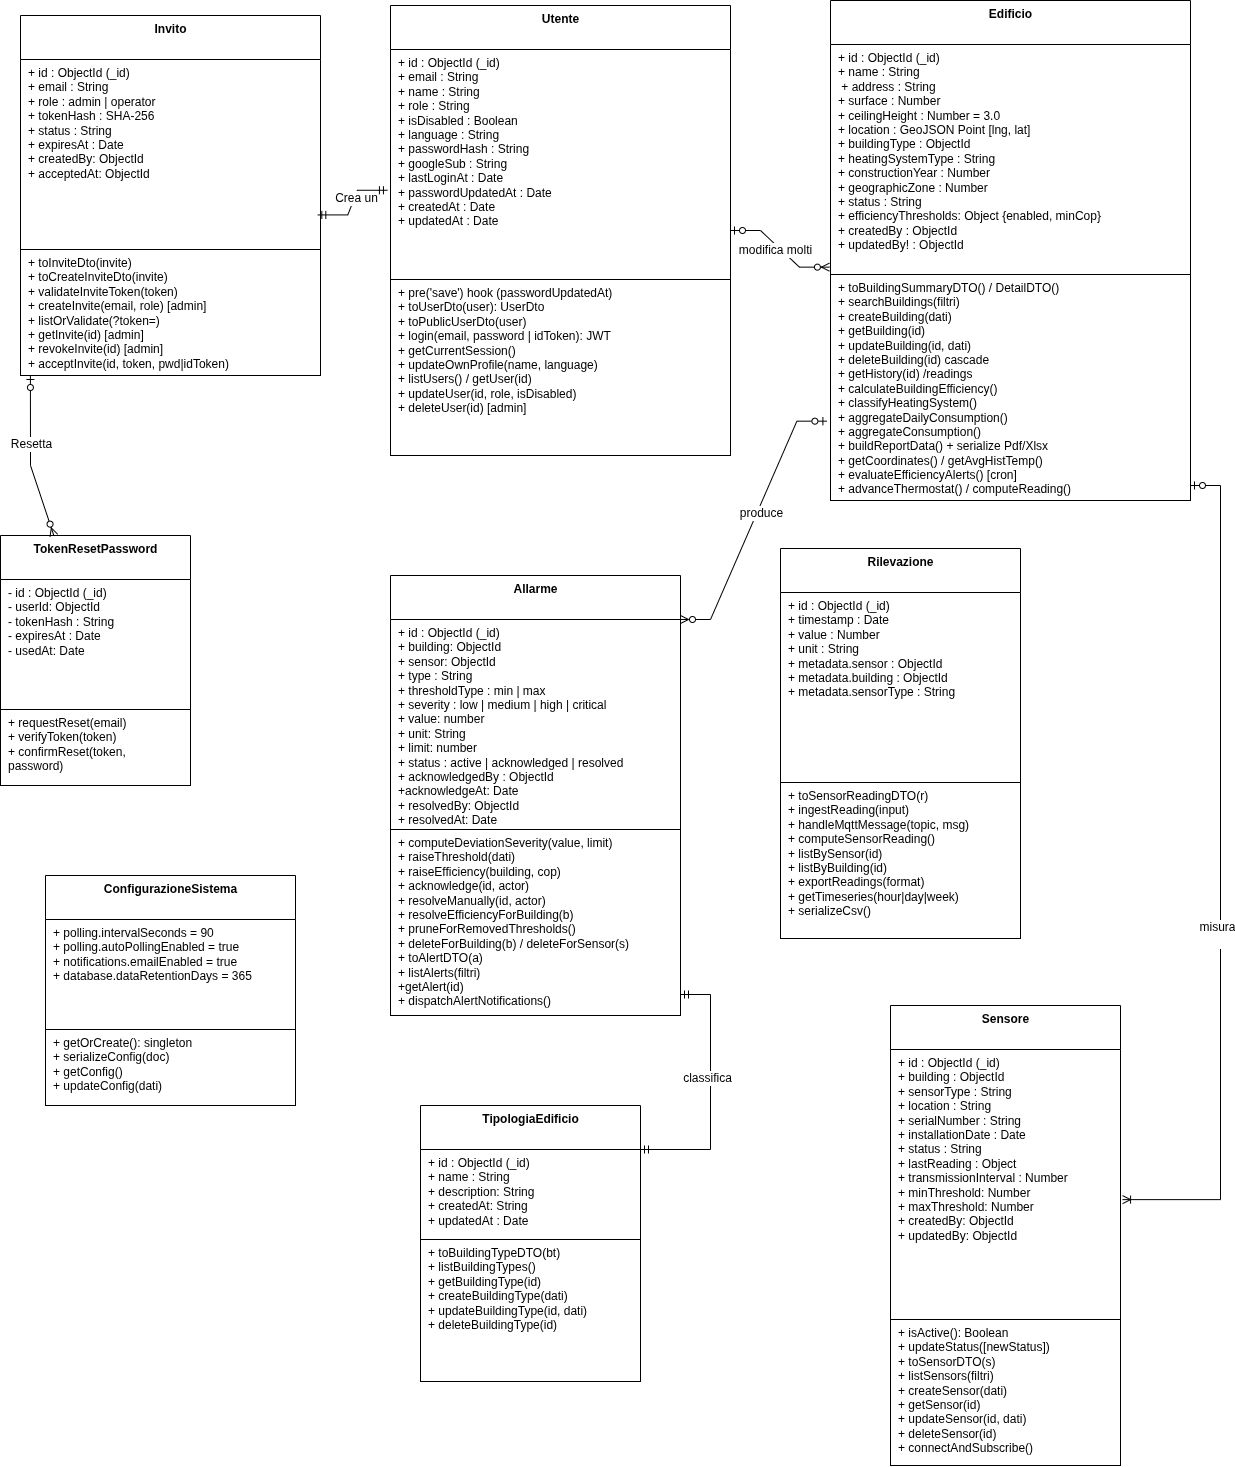
\includegraphics[width=1\textwidth]{../images/ClassDiagram/ClassiWattguard-DiagrammaGenerale.png}
        \caption{Diagramma delle classi complessivo di \texttt{WattGuard}}
    \end{figure}

\section{Dal Class Diagram alle API}
\label{ch:dalClassDiagramAlleAPI}

Riportiamo di seguito una tabella con la mappatura tra i metodi presenti nel diagramma delle classi del capitolo precedente e le API individuate nel documento D3.
L'uso del simbolo \textbf{*} indica che esso è un parametro di percorso.
Nei parametri query invece il simbolo \textbf{!} indica che il parametro è obbligatorio mentre \textbf{?} è facoltativo.

{\footnotesize
\setlength{\tabcolsep}{2.5pt}
\renewcommand{\arraystretch}{1.25}
\begin{longtable}{>{\raggedright\arraybackslash}p{2.6cm}>{\centering\arraybackslash}p{1.5cm}>{\raggedright\ttfamily\arraybackslash}p{5.6cm}>{\raggedright\arraybackslash}p{2.4cm}>{\raggedright\arraybackslash}p{2.2cm}}
\toprule
\textbf{Metodo} & \textbf{HTTP} & \textbf{URI + query} & \textbf{Request} & \textbf{Response} \\
\midrule
\endfirsthead
\toprule
\textbf{Metodo} & \textbf{HTTP} & \textbf{URI + query} & \textbf{Request} & \textbf{Response} \\
\midrule
\endhead
\bottomrule
\endfoot
\multicolumn{5}{l}{\textbf{Classe Utente --- autenticazione}} \\
\midrule
login() & POST & /auth/session & \texttt{\{email,} \allowbreak\texttt{password} \allowbreak\textbar{} \texttt{idToken\}} & \texttt{\{user,} \allowbreak\texttt{token\}} \\
get\allowbreak{}Current\allowbreak{}Session() & GET & /auth/session & - & \texttt{User} \\
update\allowbreak{}Own\allowbreak{}Profile() & PATCH & /auth/session & \texttt{\{name,} \allowbreak\texttt{language\}} & \texttt{User} \\
get\allowbreak{}Google\allowbreak{}Client\allowbreak{}Id() & GET & /auth/google/\allowbreak{}config & - & \texttt{\{clientId\}} \\
logout() & - & - & - & - \\
\midrule
\multicolumn{5}{l}{\textbf{Classe Utente --- gestione account (solo admin)}} \\
\midrule
listUsers() & GET & /users/ & - & \texttt{User[]} \\
getUser() & GET & /users/:id* & - & \texttt{User} \\
updateUser() & PATCH & /users/:id* & \texttt{\{role,} \allowbreak\texttt{isDisabled\}} & \texttt{User} \\
deleteUser() & DELETE & /users/:id* & - & 204 \\
acceptInvite() & PATCH & /invites/:id* & vedi Invito & \texttt{\{user,} \allowbreak\texttt{token\}} \\
toUserDto() & - & - & - & \texttt{User} \\
to\allowbreak{}Public\allowbreak{}User\allowbreak{}Dto() & - & - & - & \texttt{User} \\
pre('save') & - & - & - & - \\
seed\allowbreak{}Initial\allowbreak{}Records() & - & - & - & - \\
\midrule
\multicolumn{5}{l}{\textbf{Classe Invito}} \\
\midrule
createInvite() & POST & /invites/ & \texttt{\{email,} \allowbreak\texttt{role\}} & \texttt{Invite} \\
list\allowbreak{}Or\allowbreak{}Validate() & GET & /invites/ [?token=] & \texttt{?token=} & \texttt{Invite} \allowbreak\textbar{} \texttt{Invite[]} \\
getInvite() & GET & /invites/:id* & - & \texttt{Invite} \\
revokeInvite() & DELETE & /invites/:id* & - & 204 \\
acceptInvite() & PATCH & /invites/:id* & \texttt{\{token,} \allowbreak\texttt{password} \allowbreak\textbar{} \texttt{idToken\}} & \texttt{\{user,} \allowbreak\texttt{token\}} \\
validate\allowbreak{}Invite\allowbreak{}Token() & - & - & - & - \\
toInviteDto() & - & - & - & \texttt{Invite} \\
to\allowbreak{}Create\allowbreak{}Invite\allowbreak{}Dto() & - & - & - & \texttt{Invite} \\
\midrule
\multicolumn{5}{l}{\textbf{Classe TokenResetPassword}} \\
\midrule
requestReset() & POST & /auth/recovery-tokens & \texttt{\{email\}} & 200 generica \\
verifyToken() & POST & /auth/recovery-validations & \texttt{\{token\}} & \texttt{\{valid\}} \\
confirmReset() & POST & /auth/recovery-confirmations & \texttt{\{token,} \allowbreak\texttt{password\}} & 200 \\
\midrule
\multicolumn{5}{l}{\textbf{Classe Edificio}} \\
\midrule
search\allowbreak{}Buildings() & GET & /buildings/ & filtri + paginazione & \texttt{Building[]} \\
create\allowbreak{}Building() & POST & /buildings/ & anagrafica edificio & \texttt{Building} \\
getBuilding() & GET & /buildings/:id* & - & \texttt{Building} \\
update\allowbreak{}Building() & PATCH & /buildings/:id* & campi edificio & \texttt{Building} \\
delete\allowbreak{}Building() & DELETE & /buildings/:id* & - & 204 \\
getHistory() & GET & /buildings/:id*/\allowbreak{}readings \allowbreak{}?startDate!, \allowbreak{}endDate!, \allowbreak{}sensorType?, \allowbreak{}interval?, \allowbreak{}limit?, \allowbreak{}sortOrder? & - & \texttt{Reading[]} \\
getRealtime() & - & - & - & - \\
calculate\allowbreak{}Building\allowbreak{}Efficiency() & GET & /buildings/:id*/\allowbreak{}efficiency \allowbreak{}?startDate!, \allowbreak{}endDate! & - & \texttt{\{COP, ...\}} \\
build\allowbreak{}Report\allowbreak{}Data() & GET & /reports/ \allowbreak{}?buildingIds!, \allowbreak{}startDate!, \allowbreak{}endDate!, \allowbreak{}format? & - & PDF \textbar{} XLSX \\
to\allowbreak{}Building\allowbreak{}Summary\allowbreak{}DTO() & - & - & - & \texttt{Building} \\
to\allowbreak{}Building\allowbreak{}Detail\allowbreak{}DTO() & - & - & - & \texttt{Building} \\
classify\allowbreak{}Heating\allowbreak{}System() & - & - & - & - \\
aggregate\allowbreak{}Daily\allowbreak{}Consumption() & - & - & - & - \\
getCoordinates() & - & - & - & - \\
get\allowbreak{}Avg\allowbreak{}Hist\allowbreak{}Temperature() & - & - & - & - \\
evaluate\allowbreak{}Efficiency\allowbreak{}Alerts() & - & - & - & - \\
advance\allowbreak{}Thermostat() & - & - & - & - \\
compute\allowbreak{}Sensor\allowbreak{}Reading() & - & - & - & - \\
\midrule
\multicolumn{5}{l}{\textbf{Classe TipologiaEdificio}} \\
\midrule
list\allowbreak{}Building\allowbreak{}Types() & GET & /building-types/ & - & \texttt{BuildingType[]} \\
get\allowbreak{}Building\allowbreak{}Type() & GET & /building-types/:id* & - & \texttt{BuildingType} \\
create\allowbreak{}Building\allowbreak{}Type() & POST & /building-types/ & \texttt{\{name,} \allowbreak\texttt{description\}} & \texttt{BuildingType} \\
update\allowbreak{}Building\allowbreak{}Type() & PATCH & /building-types/:id* & \texttt{\{name,} \allowbreak\texttt{description\}} & \texttt{BuildingType} \\
delete\allowbreak{}Building\allowbreak{}Type() & DELETE & /building-types/:id* & - & 204 \\
to\allowbreak{}Building\allowbreak{}Type\allowbreak{}DTO() & - & - & - & \texttt{BuildingType} \\
\midrule
\multicolumn{5}{l}{\textbf{Classe Sensore}} \\
\midrule
listSensors() & GET & /sensors/ \allowbreak{}?building?, \allowbreak{}sensorType?, \allowbreak{}status? & - & \texttt{Sensor[]} \\
createSensor() & POST & /sensors/ & config. sensore & \texttt{Sensor} \\
getSensor() & GET & /sensors/:id* & - & \texttt{Sensor} \\
updateSensor() & PATCH & /sensors/:id* & config. + soglie & \texttt{Sensor} \\
deleteSensor() & DELETE & /sensors/:id* & - & 204 \\
get\allowbreak{}Sensor\allowbreak{}History() & GET & /sensors/:id*/\allowbreak{}readings \allowbreak{}?startDate?, \allowbreak{}endDate?, \allowbreak{}limit?, \allowbreak{}offset?, \allowbreak{}sortOrder? & - & \texttt{Reading[]} \\
connect\allowbreak{}And\allowbreak{}Subscribe() & MQTT & sensors/+/readings & - & - \\
isActive() & - & - & - & Boolean \\
updateStatus() & - & - & - & - \\
toSensorDTO() & - & - & - & \texttt{Sensor} \\
\midrule
\multicolumn{5}{l}{\textbf{Classe Rilevazione}} \\
\midrule
ingestReading() & MQTT & sensors/+/readings & \texttt{\{value,} \allowbreak\texttt{unit,} \allowbreak\texttt{timestamp\}} & - \\
listBySensor() & GET & /sensors/:id*/\allowbreak{}readings \allowbreak{}?startDate?, \allowbreak{}endDate?, \allowbreak{}limit?, \allowbreak{}offset?, \allowbreak{}sortOrder? & - & \texttt{Reading[]} \\
listByBuilding() & GET & /buildings/:id*/\allowbreak{}readings \allowbreak{}?startDate!, \allowbreak{}endDate!, \allowbreak{}sensorType?, \allowbreak{}interval?, \allowbreak{}limit?, \allowbreak{}sortOrder? & - & \texttt{Reading[]} \\
exportReadings() & GET & /readings/ \allowbreak{}?buildingIds?, \allowbreak{}startDate?, \allowbreak{}endDate?, \allowbreak{}format? & - & CSV \textbar{} JSON \\
getTimeseries() & GET & /metrics/\allowbreak{}timeseries \allowbreak{}?startDate!, \allowbreak{}endDate!, \allowbreak{}interval? & - & serie aggregate \\
getKpi() & GET & /metrics/ & - & KPI \\
handle\allowbreak{}Mqtt\allowbreak{}Message() & - & - & - & - \\
to\allowbreak{}Sensor\allowbreak{}Reading\allowbreak{}DTO() & - & - & - & \texttt{Reading} \\
serializeCsv() & - & - & - & CSV \\
\midrule
\multicolumn{5}{l}{\textbf{Classe Allarme}} \\
\midrule
listAlerts() & GET & /alerts/ \allowbreak{}?building?, \allowbreak{}status?, \allowbreak{}severity? & - & \texttt{Alert[]} \\
getAlert() & GET & /alerts/:id* & - & \texttt{Alert} \\
acknowledge() & PATCH & /alerts/:id* & \texttt{\{status:} \allowbreak\texttt{acknowledged\}} & \texttt{Alert} \\
resolve\allowbreak{}Manually() & PATCH & /alerts/:id* & \texttt{\{status:} \allowbreak\texttt{resolved\}} & \texttt{Alert} \\
raise\allowbreak{}Threshold() & - & - & - & \texttt{Alert} \\
raise\allowbreak{}Efficiency() & - & - & - & \texttt{Alert} \\
resolve\allowbreak{}Efficiency\allowbreak{}ForBuilding() & - & - & - & - \\
prune\allowbreak{}ForRemoved\allowbreak{}Thresholds() & - & - & - & - \\
delete\allowbreak{}ForBuilding() & - & - & - & - \\
delete\allowbreak{}ForSensor() & - & - & - & - \\
compute\allowbreak{}Deviation\allowbreak{}Severity() & - & - & - & \texttt{severity} \\
toAlertDTO() & - & - & - & \texttt{Alert} \\
dispatch\allowbreak{}Alert\allowbreak{}Notifications() & - & - & - & - \\
\midrule
\multicolumn{5}{l}{\textbf{Classe ConfigurazioneSistema}} \\
\midrule
getConfig() & GET & /settings/ & - & \texttt{Config} \\
updateConfig() & PATCH & /settings/ & \texttt{\{polling,} \allowbreak\texttt{notif.,} \allowbreak\texttt{database\}} & \texttt{Config} \\
downloadBackup() & GET & /backups/ & - & JSON download \\
get\allowbreak{}Or\allowbreak{}Create() & - & - & - & \texttt{Config} \\
serialize\allowbreak{}Config() & - & - & - & \texttt{Config} \\
\end{longtable}
}

\end{document}